\documentclass[10pt,a4paper]{article}
\usepackage[margin=1.4cm]{geometry}
\usepackage{helvet}\renewcommand{\familydefault}{\sfdefault}
\usepackage{graphicx,booktabs,xcolor,fancyhdr,multicol,float}
\definecolor{bigorange}{RGB}{255,130,0}
\definecolor{biggrey}{RGB}{60,60,60}
\pagestyle{fancy}\fancyhf{}
\lhead{\textbf{\color{bigorange}Banco BIG} \color{biggrey}| Rates Research}
\rhead{\color{biggrey}\today}
\renewcommand{\headrulewidth}{1pt}
\setlength{\parindent}{0pt}\setlength{\parskip}{4pt}
\begin{document}
\begin{center}
{\Large\textbf{\color{biggrey}Why Don't Rates Move With Oil?}}\\[2pt]
{\color{bigorange}\rule{\textwidth}{2pt}}\\[2pt]
{\small A conditional-sensitivity study: US10Y vs WTI, 1986--2026 daily (FRED, free data).}
\end{center}

\textbf{\color{bigorange}1. The puzzle, quantified}\\
Both series are I(1); everything below runs on oil log-returns vs bp changes. The full-sample daily
sensitivity is \textbf{+0.26bp per 1\% oil} (HAC $t$=6.6) — statistically real but
economically tiny: $R^2$ = 1.4\%, so a 5\% oil move maps to $\approx$1.3bp on the 10Y.
Monthly: +0.36bp ($t$=2.6); Brent robustness: +0.23bp ($t$=6.3).

\begin{figure}[H]\centering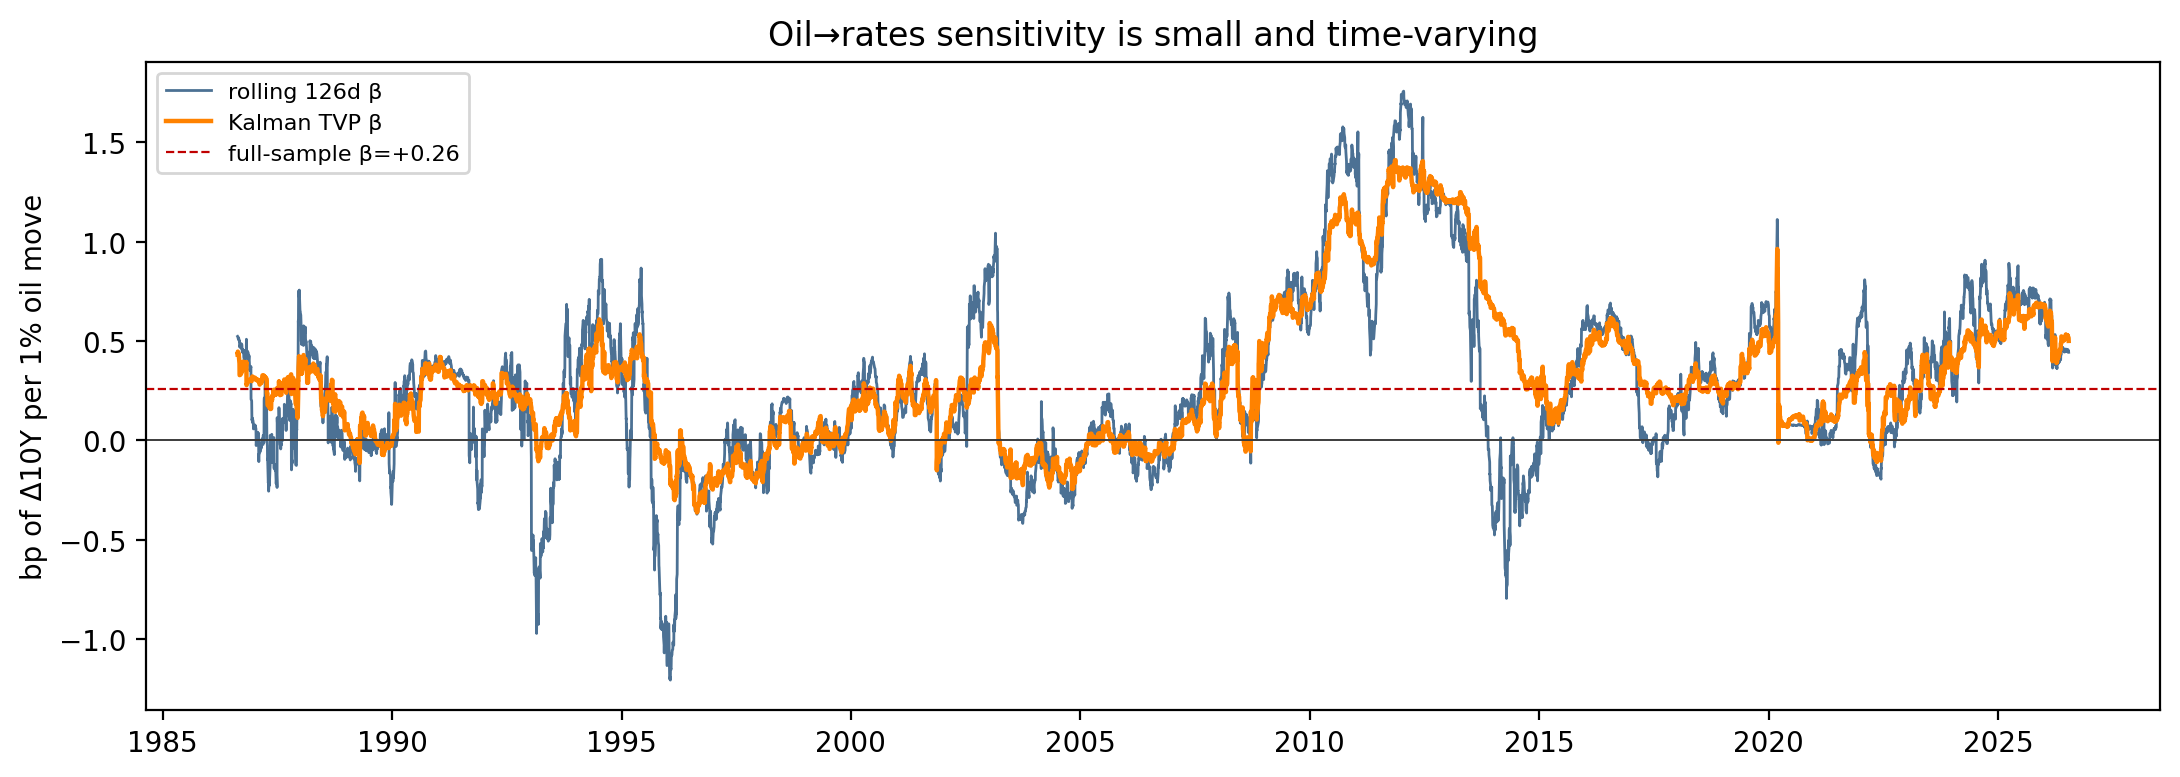
\includegraphics[width=0.98\textwidth]{fig_beta_timeline.png}\end{figure}

\textbf{\color{bigorange}2. The mechanism: two channels that offset}\\
Nominal = real + breakeven. Oil's effect runs \emph{entirely} through the inflation leg:
oil$\to$breakeven $\beta$=+0.27 ($t$=4.2, $R^2$=5.3\%);
oil$\to$real $\beta$=+0.02 ($t$=0.4, $\approx$0). Granger confirms:
oil$\to$BEI p=0.004, oil$\to$real p=0.44.
On big-oil days ($|$ret$|>$3\%, n=737) the real and breakeven legs move in \textbf{opposite
directions 60\% of the time} (corr -0.32) and the real leg is
\emph{larger} on average ($|\Delta$real$|$=4.7bp vs $|\Delta$bei$|$=3.5bp)
— the growth/risk channel cancels the inflation channel exactly when oil moves most.

\begin{figure}[H]\centering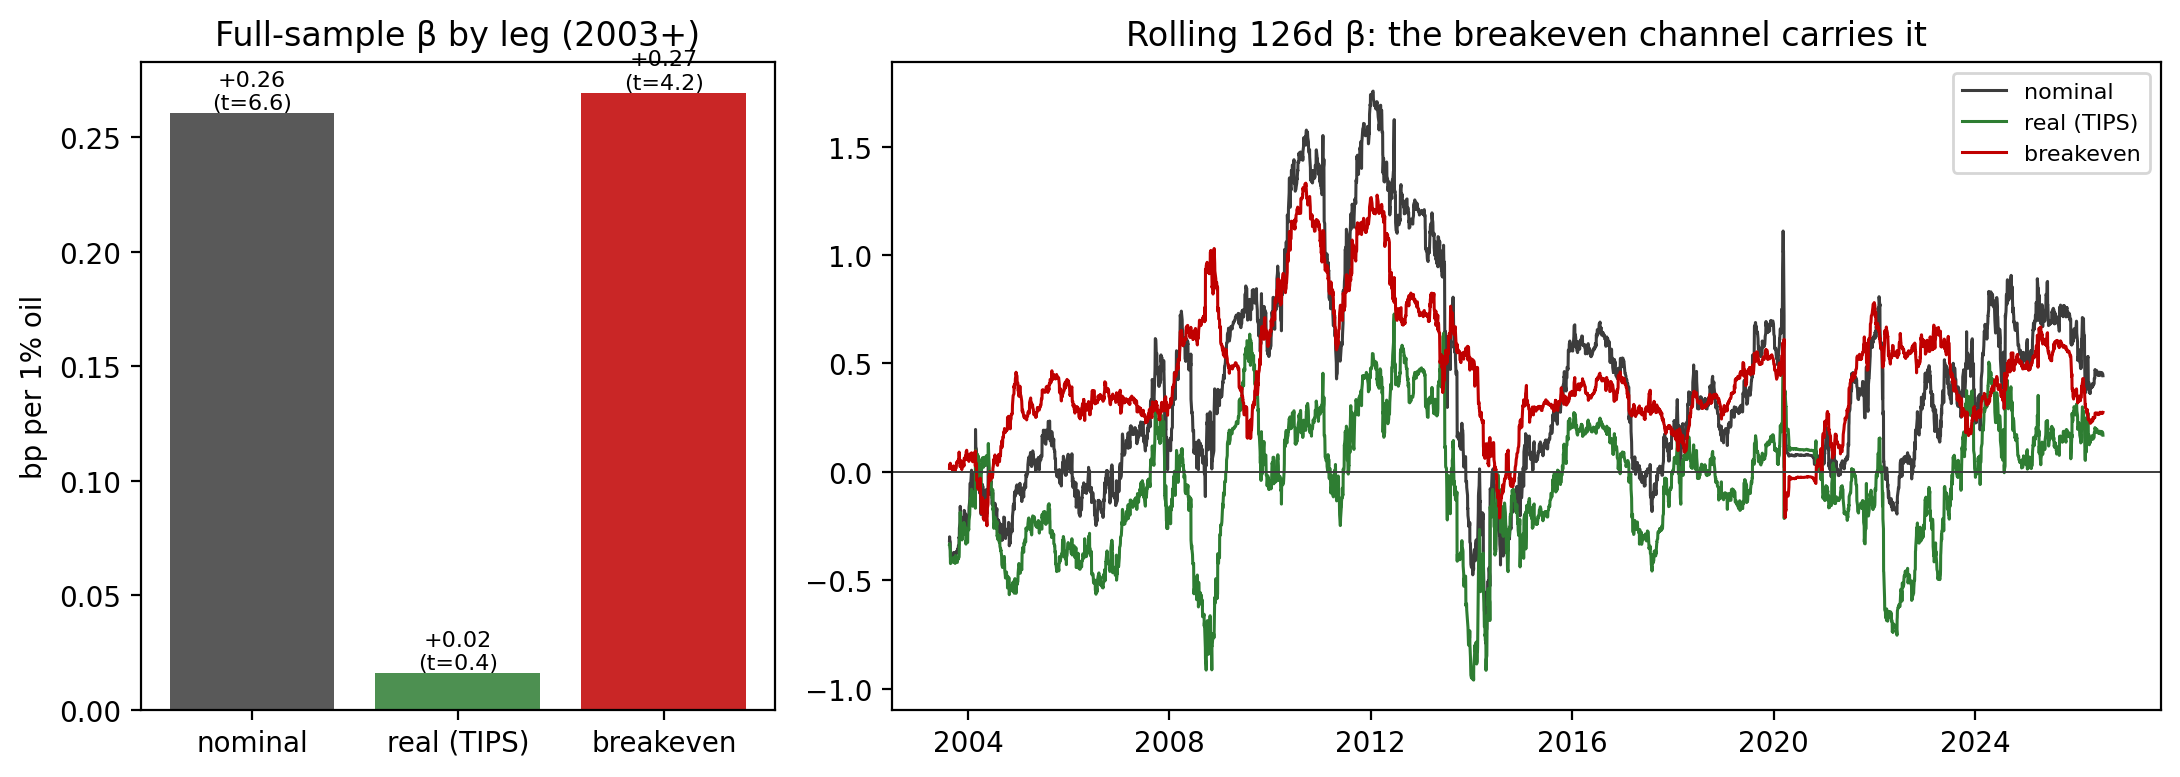
\includegraphics[width=0.98\textwidth]{fig_decomposition.png}\end{figure}

\textbf{\color{bigorange}3. The conditions for low sensitivity (regimes)}\\
A 2-state Markov-switching regression finds a \textbf{low-sensitivity state}
($\beta$=+0.21, 37\% of days) that is the \emph{high-stress} state:
VIX 23 vs 17, oil vol
2.6 vs 2.1\%/d, rate vol
7.5 vs 4.5bp/d (all p$<$0.01);
the calm state carries $\beta$=+0.33. The only significant interaction is
\textbf{oil volatility} ($t$=-5.0): per-unit sensitivity \emph{halves}
as oil vol doubles — the response \textbf{saturates}, so exactly when oil moves most (supply shocks,
risk-off), each 1\% carries the least rate signal. In bp terms the two states respond similarly
($\beta\times$typical move $\approx$ 0.5 vs
0.7bp/day).

\begin{multicols}{2}
\begin{figure}[H]\centering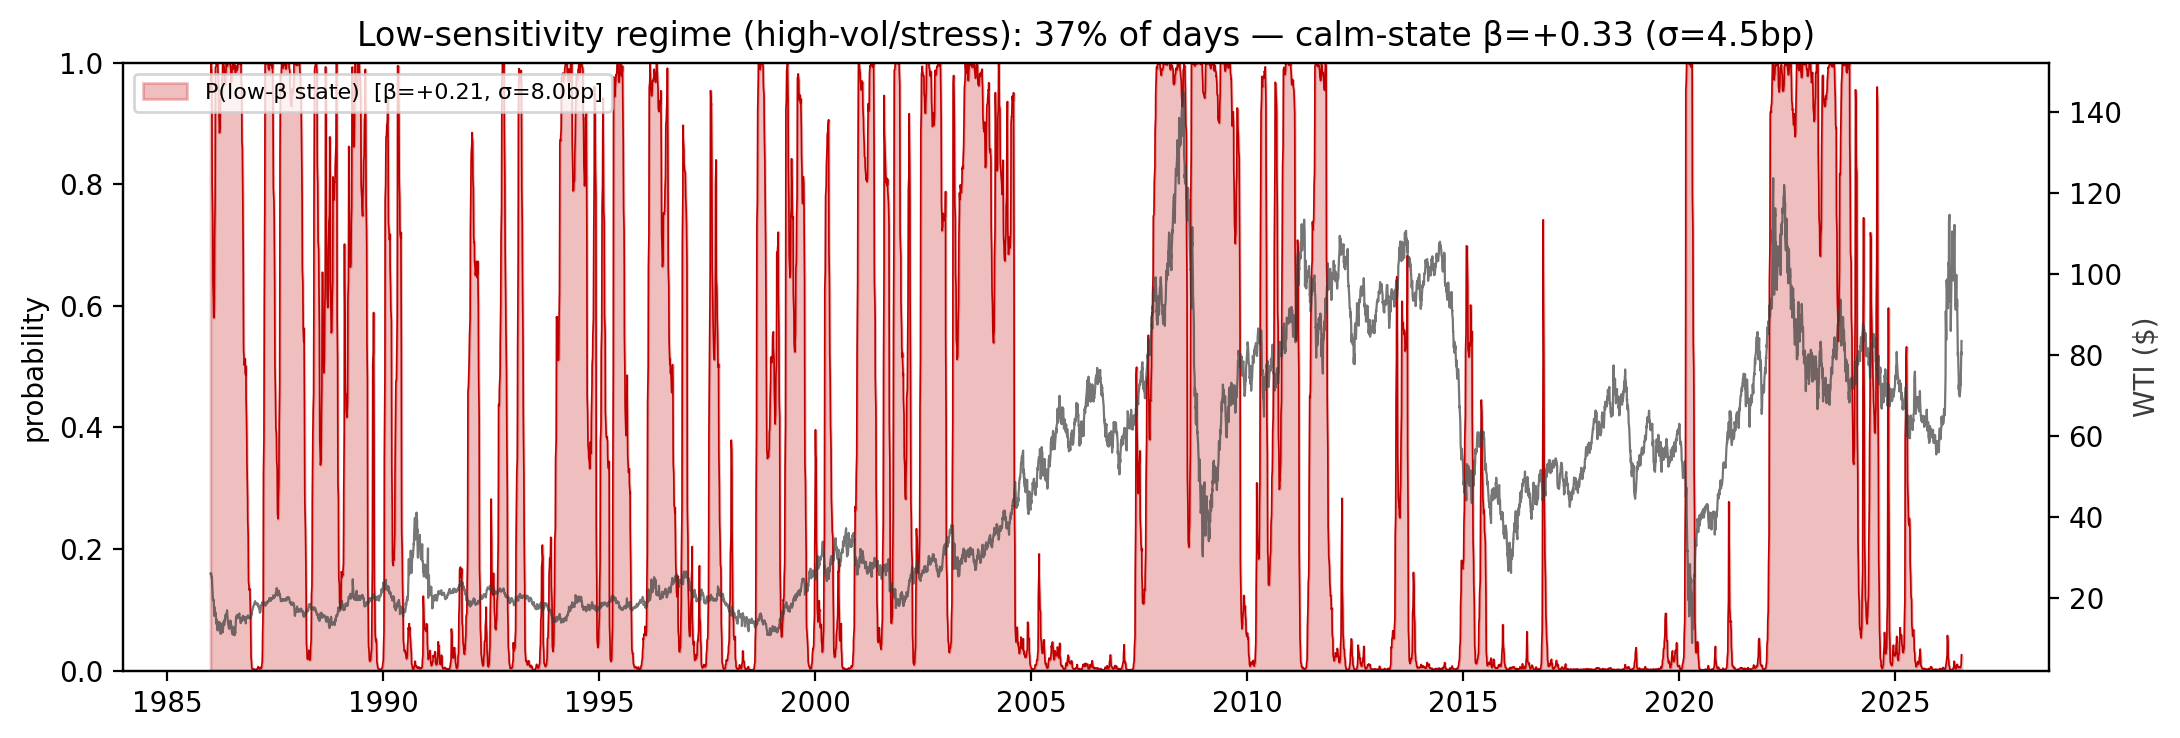
\includegraphics[width=\linewidth]{fig_markov.png}\end{figure}
\begin{figure}[H]\centering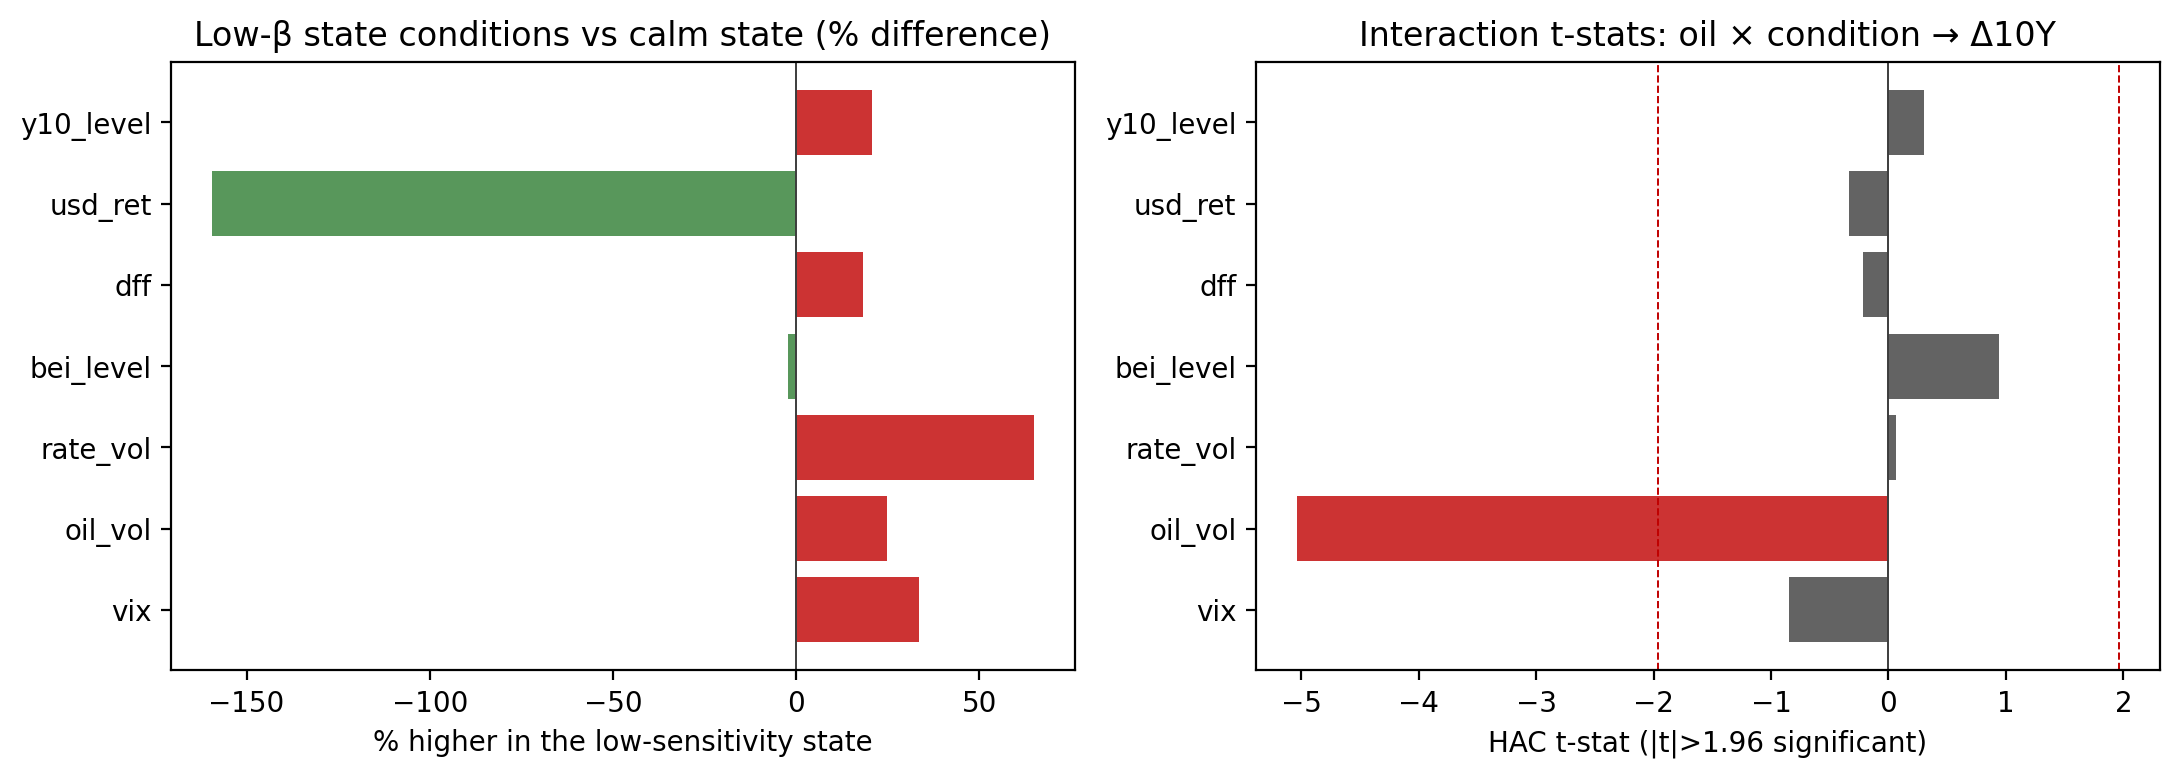
\includegraphics[width=\linewidth]{fig_conditions.png}\end{figure}
\end{multicols}

\textbf{\color{bigorange}4. The datapoints that skew the distribution}\\
The influential tail is a handful of supply/panic days — 2020-04-21 (oil -72\%,
rates -5bp), the Mar-2020 COVID cluster, 17-Jan-1991 (Gulf War), Nov-2008 — where rates
decoupled or moved \emph{against} oil. They \textbf{drag the unconditional $\beta$ down}: OLS
+0.26 $\to$ +0.30 excluding the top-1\% Cook's-D days
(robust Huber +0.27). Conditional on $|$oil$|>$5\% (n=349),
the mean rate move is -0.7bp — effectively zero.

\begin{multicols}{2}
\begin{figure}[H]\centering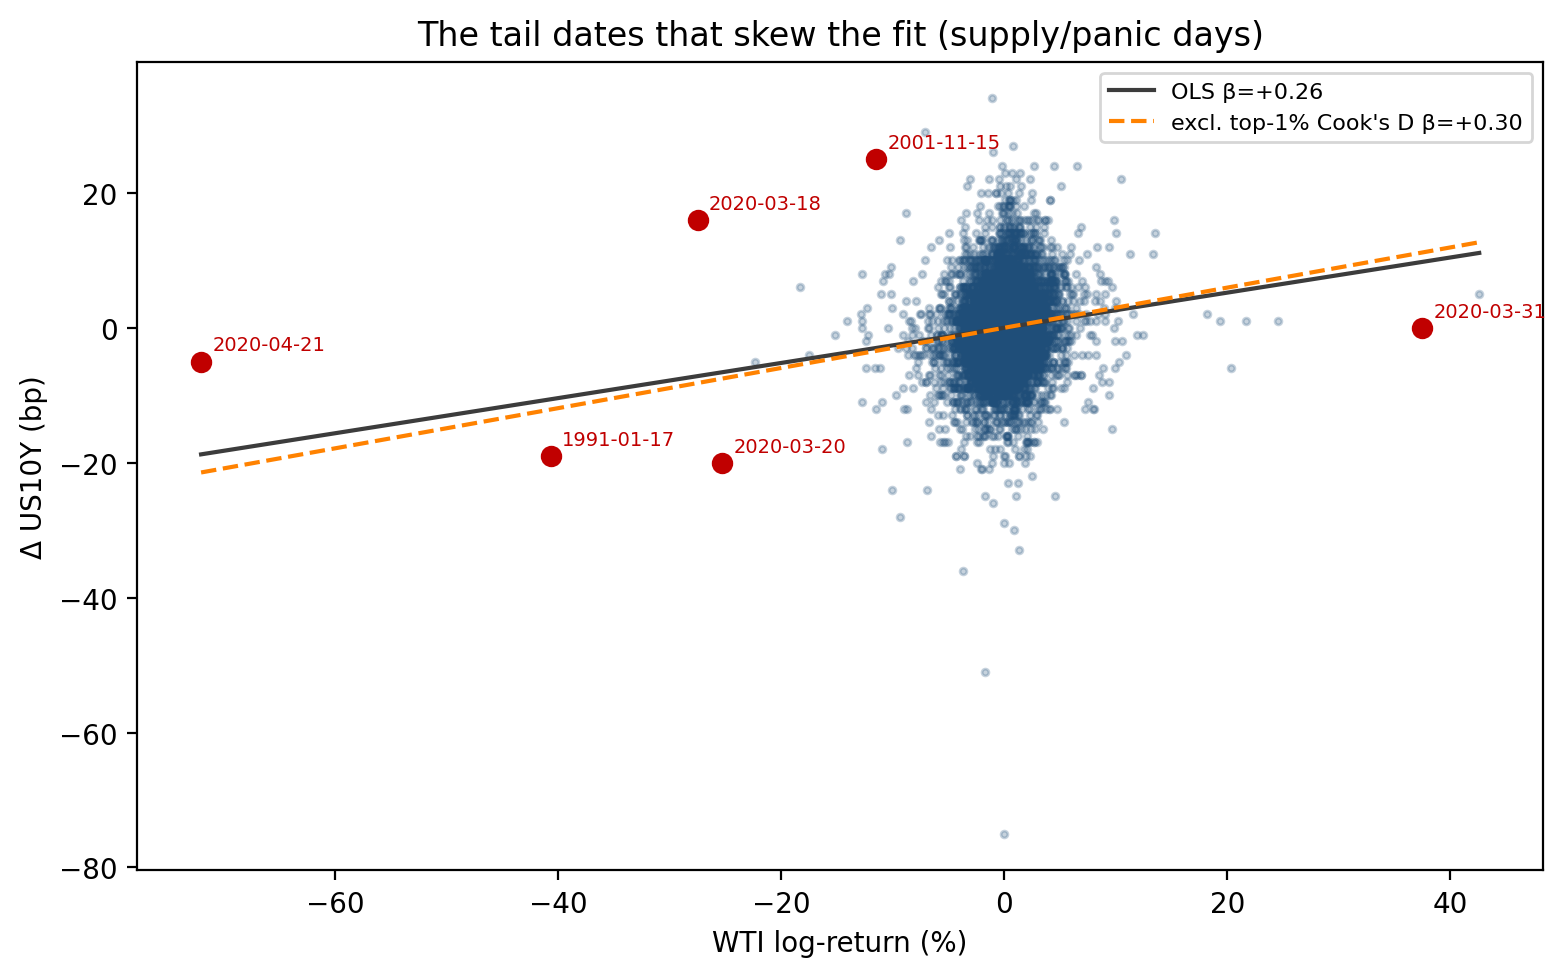
\includegraphics[width=\linewidth]{fig_influence.png}\end{figure}
\begin{figure}[H]\centering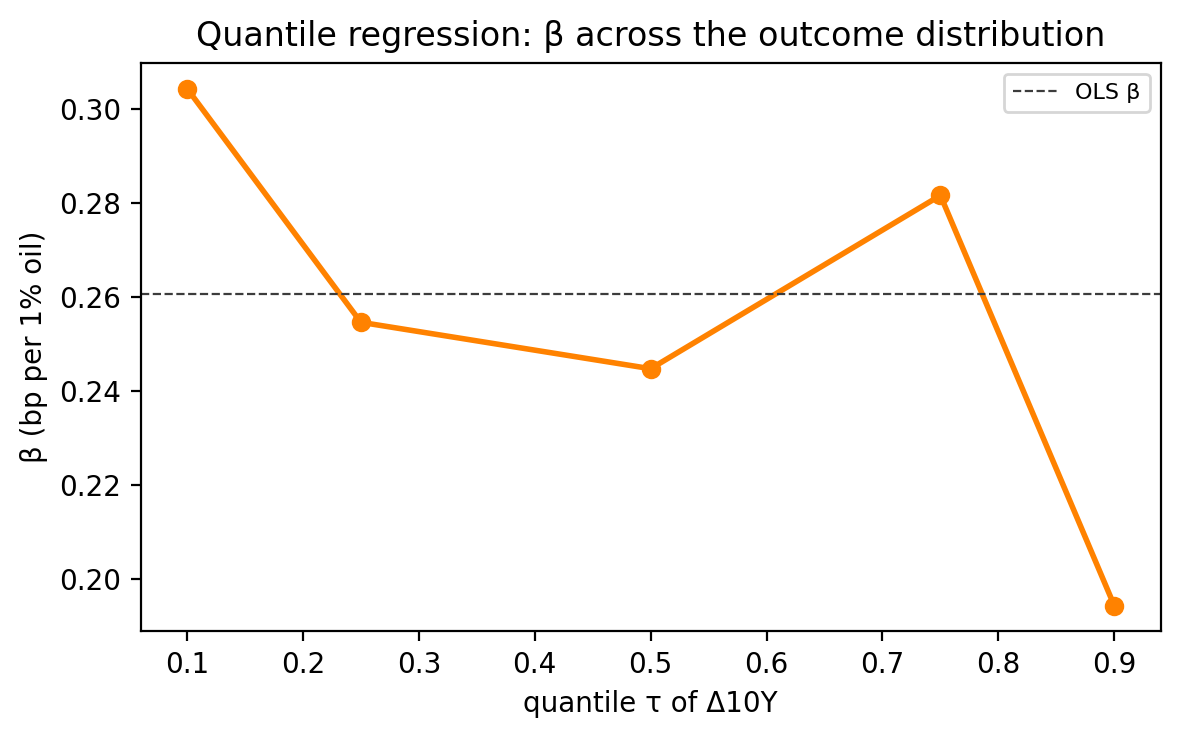
\includegraphics[width=\linewidth]{fig_quantile.png}\end{figure}
\end{multicols}

\textbf{\color{bigorange}5. Demand vs supply shocks: sign identification}\\
Classifying each day by same-day S\&P~500 co-movement (oil and equities together = \textbf{demand}
shock, opposite = \textbf{supply} shock; 2479 days
2016--2026, 55\% demand /
45\% supply — the free equity history caps the sample at $\sim$10y):
on \textbf{demand days} oil$\to$10Y $\beta$=+0.21 ($t$=2.6),
carried by the breakeven leg ($\beta$=+0.19, $t$=2.0; real
$\beta$=+0.02, $t$=0.4). On \textbf{supply days} \emph{no}
leg is significant: nominal $\beta$=+0.13 ($t$=1.6), breakeven
$\beta$=+0.06 ($t$=0.7). The ordering matches the demand-shock
hypothesis and holds on big-oil days ($|$oil$|>$2\%: demand $t$=2.6
vs supply $t$=1.3) — but honestly stated, the demand--supply
gap in $\beta$ is \emph{modest} (+0.21 vs +0.13bp per 1\%),
not dramatic: the sharper distinction is significance, not size. Most recent 21
classified days (2026-06-18--2026-07-20): 9 demand / 12 supply
$\to$ a \textbf{mixed} tape, so the current oil impulse should be read with the (weaker)
supply-day betas in mind.

\begin{figure}[H]\centering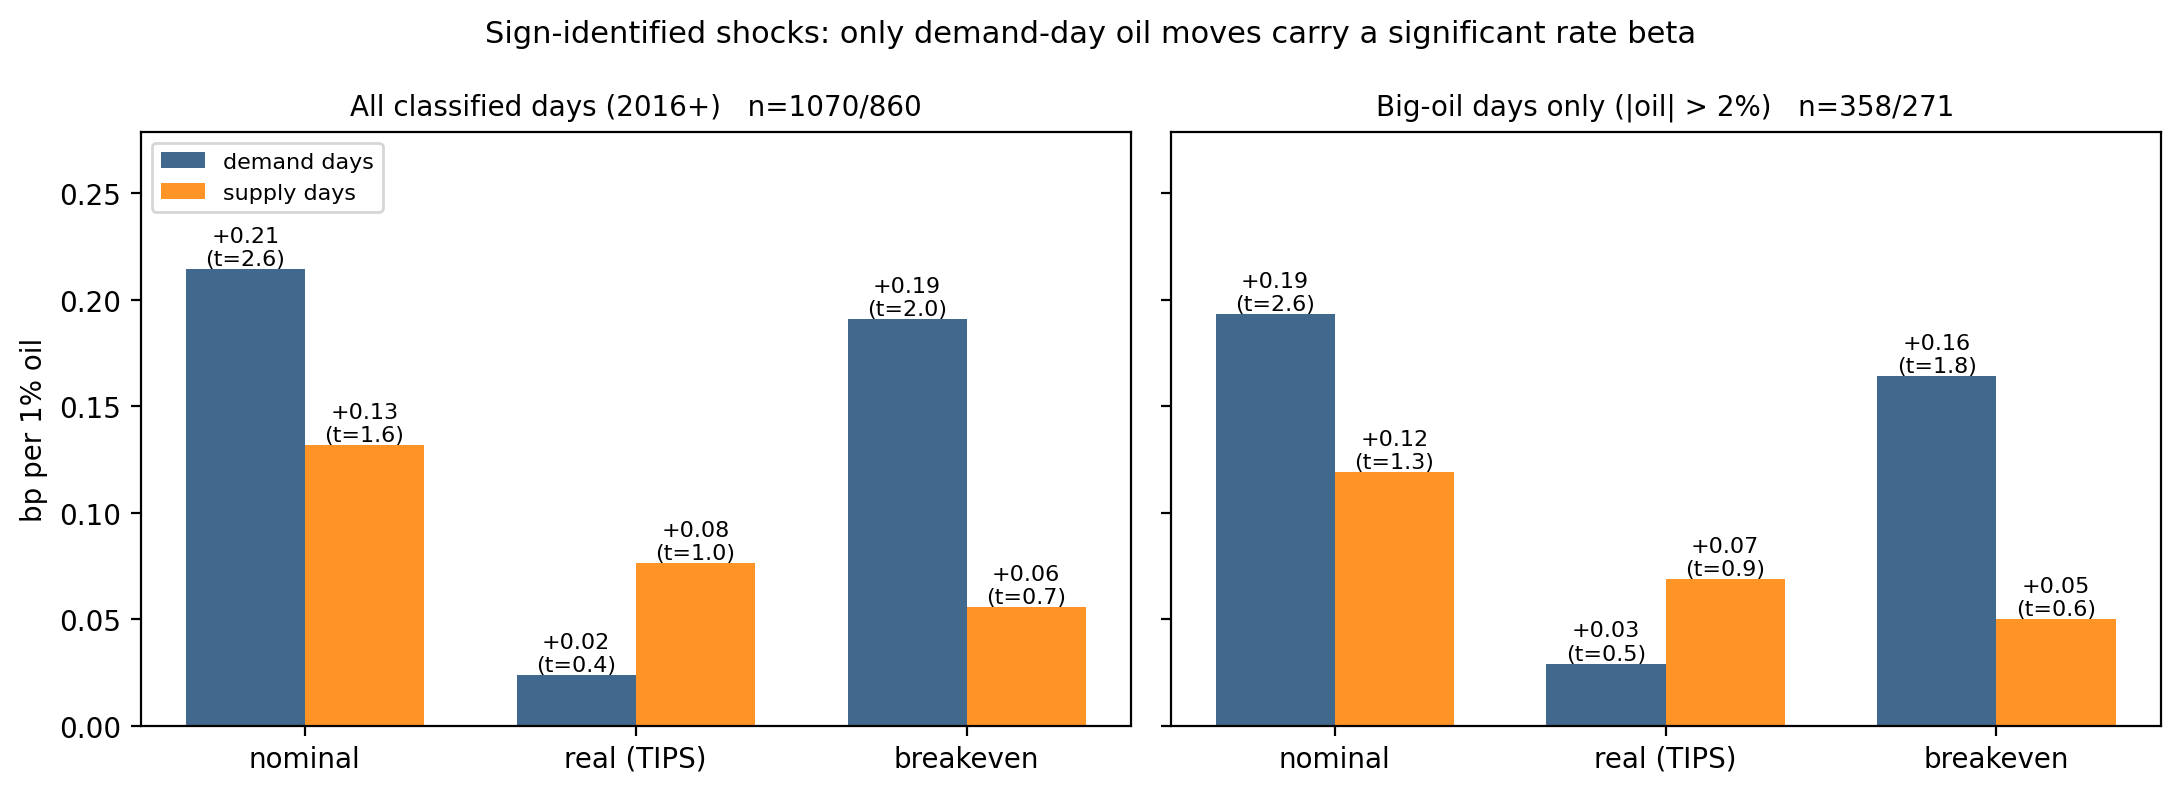
\includegraphics[width=0.98\textwidth]{fig_shock_type.png}\end{figure}

\textbf{\color{bigorange}Bottom line}\\
Rates ``don't move with oil'' because (i) the pass-through runs only through breakevens and is small
($\approx$0.3bp per 1\%), (ii) in stress/supply-shock regimes the real-rate (growth) leg moves opposite
to the inflation leg and cancels it — and that is precisely when oil moves most, (iii) per-unit
sensitivity saturates with oil volatility, and (iv) the unconditional estimate is further dragged down by
a few identifiable panic days. Oil matters for \emph{breakeven} positioning; for nominal duration it is
a second-order input unless the move is demand-led in a calm regime.

\vspace{4pt}{\footnotesize\color{biggrey}Sources: FRED (DCOILWTICO, DCOILBRENTEU, DGS10, DFII10,
T10YIE, VIXCLS, DTWEXBGS, DFF, SP500). WTI negative-price day 2020-04-20 excluded from returns.
HAC/Newey-West errors; Markov 2-state ML; Cook's-distance influence; Kilian-style sign identification
for demand/supply days. Reproduce: \texttt{python -m oil\_rates.run --report}.}
\end{document}
